\subsection{LGAD検出器の電流電圧特性を用いた温度測定}
レーザー測定で使用する装置は、恒温層よりも大きいので、恒温層を使ったセンサーとアンプボードの温度調節・測定ができない。
%そのため、ペルチェとチラーによる空冷で使用するセンサーとアンプボードの温度上昇を抑制している。
そのため、20${}^\circ$Cに設定した恒温層内のLGADの電流電圧特性と、今回の測定セットアップ内での電流電圧特性を比較することで、測定系の温度を調べた。
今回の電流電圧特性の測定では、2 Vステップで暗電流が100 $\mu\rm{A}$になるまで行った。
図\ref{fg:IV_temp} にLGADの電流電圧特性の測定結果を示す。
青のデータ点がレーザーのセットアップ内で測定した電流電圧特性で、赤のデータ点が恒温層内で測定した電流電圧測定である。
LGAD検出器の降伏電圧は、1${}^\circ$C増加すると1.1 V増える\cite{Kita_Master}。
暗電流の上昇率が初めて 10 倍を超えた点を降伏電圧をすると、
レーザーのセットアップ内での降伏電圧が198 Vで恒温層内での降伏電圧が186 Vであった。
そのため、今回の実験セットアップでは、降伏電圧が12 V増加していることがわかった。
よって、本実験の測定系では、センサーが32${}^\circ$Cであると考えられる。

\begin{figure}[h]
        \centering
        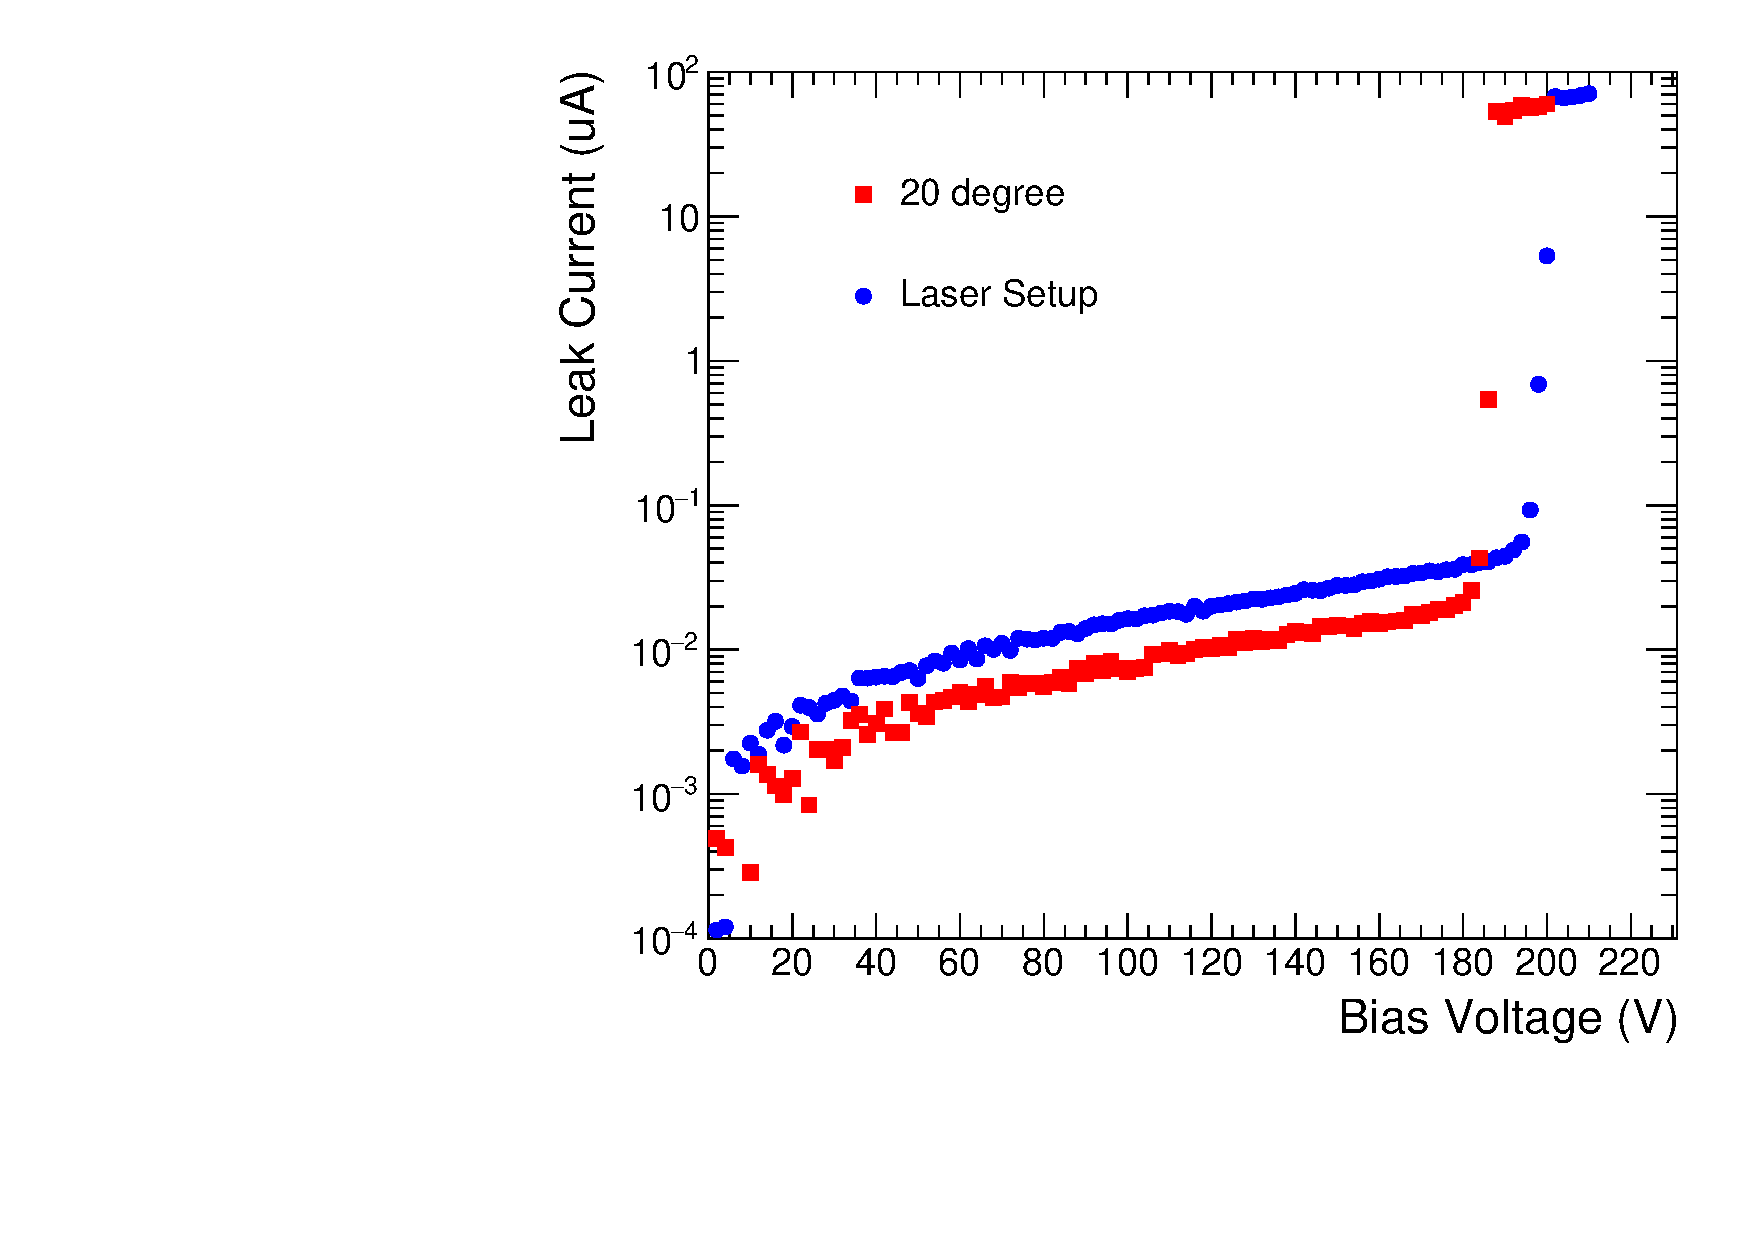
\includegraphics[width=8cm]{fig/graph/IV_20degree_Lasersetup.pdf}
        \caption[AC-LGAD検出器の電流電圧特性]{AC-LGAD検出器の電流電圧特性\\恒温層内で測定した電流電圧特性(赤)とレーザーセットアップで測定した電流電圧特性(青)の比較}
        \label{fg:IV_temp}
\end{figure}


%また、電子雪崩を起こす前の領域での暗電流の変化からも温度を見積もることができる。電子雪崩を起こす前の領域では、7.7${}^\circ$Cで2倍に上昇することがわかっている。この領域では暗電流はレーザーセットアップと恒温層で2倍の差があった。そのため、この領域から約28${}^\circ$Cであることが見積もれる。
%温度の見積もりの方法で温度に差が生じた理由は、

%剥離した後のサンプルが正常に動作するかを調べるため、に電流電圧特性を測定した。今回の測定では2Vステップで暗電流が100 $\mu\rm{A}$になるまで測定を行った。
%以下の図\ref{fg:IV_ething}にAPDの電流電圧特性の測定結果を示す。
%グラフの青点が剥離前のサンプルで赤点が剥離後のサンプルの電圧電流特性である。暗電流が0V~180Vまで一定で190V付近で電子雪崩による急激に上昇することがわかる。

%図\ref{fg:IV_ething}の2つのデータを比較すると、剥離後は剥離前と比べて0V~180Vでの暗電流の上昇を約10倍ほどになった。
%この暗電流の上昇は酸化膜の除去の影響であると考える。ピンセットで酸化膜を除去した際は暗電流が約1000倍になったので、
%ワイヤーボンディングのウェッジを使うことで暗電流の上昇を約10倍まで抑えることができたと考える。
%190V付近の電子雪崩を起こす領域についてはほとんど同じ電流電圧特性を持つサンプルを作成することができた。